\documentclass[output=paper]{langsci/langscibook} 
\author{Isabelle Udry\orcid{}\affiliation{University of Fribourg, Institut de Plurilinguisme; Zurich University of Teacher Education} and Raphael Berthele\orcid{}\affiliation{University of Fribourg, Institut de Plurilinguisme}}
\title[The smart, the motivated and the self-confident]
      {The smart, the motivated and the self-confident: The role of language aptitude, cognition, and affective variables in early instructed foreign language learning}
\abstract{We investigated the underlying structure of language-related, cognitive, and affective variables assessed in a test battery. First, we conducted an exploratory factor analysis (EFA) with data from LAPS I (174 learners of L2 French, mean age 11.1). Second, we conducted a confirmatory factor analysis (CFA) with data from LAPS~II (615 learners of L2 English, mean age 10.5). EFA with LAPS I data yielded an optimal solution with three dimensions: (1) General cognitive abilities and language aptitude (Cognition/Aptitude Factor); (2) extrinsic motivation, dedication, parental and teacher encouragement (Extrinsic Factor); (3) intrinsic motivation, foreign language anxiety, and L2 self-concept (L2 Academic Emotion Factor). The CFA with sample LAPS II validated the EFA factor structure. The findings provide robust evidence for a cognitive dimension involving language aptitude, IQ, working memory, field independence and language of instruction, even when context and L2 differ. 

A regression analysis was carried out with the 3 factors as predictors and L2 proficiency as the dependent variable. It reveals that Factor 1 (Cognition/Aptitude) and Factor 3 (L2 Academic Emotion) are positively associated with L2 proficiency. When the two other factors are controlled for, a negative effect of the Extrinsic Factor on L2 proficiency is observed in the data.}
\IfFileExists{../localcommands.tex}{
  \addbibresource{localbibliography.bib}
  % add all extra packages you need to load to this file

\usepackage{tabularx,multicol}
\usepackage{url}
\urlstyle{same}

\usepackage{listings}
\lstset{basicstyle=\ttfamily,tabsize=2,breaklines=true}

%\usepackage{langsci-optional}
\usepackage{langsci-lgr}
\usepackage{langsci-gb4e}
\usepackage{langsci-optional}

\usepackage{enumitem}
\usepackage[group-digits=false, detect-weight=true]{siunitx}

\usepackage{todonotes}

  \newcommand*{\orcid}{}
 
  %% hyphenation points for line breaks
%% Normally, automatic hyphenation in LaTeX is very good
%% If a word is mis-hyphenated, add it to this file
%%
%% add information to TeX file before \begin{document} with:
%% %% hyphenation points for line breaks
%% Normally, automatic hyphenation in LaTeX is very good
%% If a word is mis-hyphenated, add it to this file
%%
%% add information to TeX file before \begin{document} with:
%% %% hyphenation points for line breaks
%% Normally, automatic hyphenation in LaTeX is very good
%% If a word is mis-hyphenated, add it to this file
%%
%% add information to TeX file before \begin{document} with:
%% \include{localhyphenation}
\hyphenation{
affri-ca-te
affri-ca-tes 
Soa-res
scru-ti-ny
me-ta-cog-ni-tion
}

\hyphenation{
affri-ca-te
affri-ca-tes 
Soa-res
scru-ti-ny
me-ta-cog-ni-tion
}

\hyphenation{
affri-ca-te
affri-ca-tes 
Soa-res
scru-ti-ny
me-ta-cog-ni-tion
}
 
  \togglepaper[1]%%chapternumber
}{}

\begin{document}
\maketitle 

\section{Introduction}

The goal of this chapter is to explore the relationship between individual differences (IDs) and their impact on L2 learning outcomes. To this aim, we administered a test battery of language-related, cognitive, and affective variables to primary school children aged 10--12 years, learning foreign languages as part of the mandatory curriculum. The conceptual framework of these variables is discussed in Chapter 1, a full description of the test battery can be found in Chapter 2. The following research questions were addressed:

\begin{enumerate}
\item  What is the underlying structure of the ID variables, particularly in relation to language aptitude and general cognitive abilities?
\item  Is the structure replicable in an independent sample?
\item  What are the effects of the ID variables on L2 proficiency?
\end{enumerate}

Chapter 4 deals with predictive models involving all IDs and environmental factors assessed in the LAPS project, and Chapter 5 considers the impact of environmental factors. This chapter is concerned with the latent constructs pertaining to the individual only and their relationship with instructed foreign language learning. A better understanding of these questions can inform curricular planning. 

\section{Design and Procedure} %%%\footnote{We summarize the relevant points for this chapter. Full details on procedure, participants, and test instruments are given in Chapter 2.}

To describe patterns of IDs as they emerge from the data, we adopted a data-driven approach based on recommendations by \citet{Brown2006}. The factor analysis was conducted in two steps: In step 1, we performed an exploratory factor analysis (EFA) on the sample from LAPS I (first data collection T1, L2 learners of French). In step 2, we applied confirmatory factor analysis (CFA) to the data from LAPS II (first data collection T1, L2 learners of English). Finally, a regression analysis was carried out with both samples with L2 proficiency as the dependent variable. This procedure allowed for a maximally unbiased approach to the data. 

As one of the reviewers rightly pointed out, other statistical procedures involve testing pre-specified, theory-based models with the same data and then deciding on the most appropriate model, according to goodness-of-fit indices and theoretical assumptions. Since we did not intend to test a specific theory of language learning this approach seemed less suitable for our context. Moreover, as outlined in Chapter 4, it is not uncommon for several competing models to yield an acceptable goodness-of-fit. Statistical analysis that starts with applying different theory-based models to the same sample, to our mind, bears the risk of circular thinking whereby a theory that has not been fully validated (and that the study may intend to test) is eventually used to corroborate this theory, even though other models may also have performed within an acceptable range\footnote{For a discussion, see for instance \citet{VafaeeEtAl2017} on modelling measures of explicit versus implicit L2 knowledge.}. We therefore chose the procedure described above which we deemed to be most appropriate for our descriptive approach and our research questions.

\subsection{Sample}

Native speakers of French and English were excluded from the samples. As such participants cannot be considered L2 learners of the respective languages, their answers in the questionnaire assessing motivation for L2 learning were expected to be incongruent with those of L2 learners. Incomplete data points were also removed from the data. This resulted in the following datasets:

The exploratory factor analysis was conducted with data from LAPS I which consists of 174 L2 French learners, mean age 11.1 years (4\textsuperscript{th} and 5\textsuperscript{th} grade) with L1 German. The data were collected in 2017 in 10 classes located close to the French-speaking part of Switzerland. These children started to learn L2 French in 3\textsuperscript{rd} grade at age 9. 

The confirmatory factor analysis was conducted with data from LAPS II and consists of 615 L2 English learners, mean age 10.5 years (4\textsuperscript{th} and 5\textsuperscript{th} grade) with L1 German. Data collection took place in autumn 2017 in the Swiss German speaking part of the country in 32 classes. Children from this sample had already started with L2 English lessons in 2nd grade. 

\subsection{Test instruments} 

A test battery including measures of language aptitude, cognition, and affective variables was compiled and administered on 4 lessons of 45 minutes distributed over 2 sessions on different days.\footnote{Full details on the test battery are given in Chapter 2.}

\subsubsection{Language aptitude}

\begin{description}
\item[Inductive ability (ind):] Participants are presented with words and short sentences in an artificial language, as well as their translation in the school language. The participants’ task is to infer regularities and translate sentences following the same pattern from the school language into the artificial language. This is inspired by a task (Form 4) of the Pimsleur language aptitude battery (PLAB; \citealt{Pimsleur1966}). Task design (structure of the artificial language and instructions) was customized to fit our target group.

\item[Grammatical sensitivity (gra):] Participants are presented with two sentences. In the first one, a word is highlighted. The participants’ task is to find, in the second sentence, the word having the same function as the highlighted word in the first sentence. This task is based on Part 2 (‘Matching Words’) of the Modern Language Aptitude Test - Elementary (MLAT-E; \citealt{CarrollSapon1976}) and was presented in the language of instruction, German.

\item[Phonetic coding ability (pho):] We used two subtests of \citegen{MearaEtAl2001} Llama test battery.

\begin{itemize}
\item In the LLAMA E (sound-symbol association), participants have two minutes to learn how sounds are spelled in an artificial language (training phase). Their task is then to listen to bi-syllabic words in the artificial language and pick their correct spelling from among two options (used in LAPS I).
\item LLAMA D (phonemic discrimination): In a trial phase, participants hear different sounds. During testing, they listen to strings of sounds and are asked to identify the sounds from the trial phase (used in LAPS II).
\end{itemize}
\end{description}

\subsubsection{General learning abilities}

\begin{description}
\item[Intelligence (iq):] CFT 20-R \citep{Weiss2006}. The participants complete number sequences (LAPS I) and matrices/topological deduction (LAPS II).

\item[Field (in-)dependence (fie):] In the Group Embedded Figures test (GEFT, Witkin et al. 2014), participants have to find simple geometrical figures embedded in more complex figures under time pressure.

\item[Working memory:]
\begin{itemize}
\item[]
\item \textit{Visuospatial working memory (vis):} We administered an adaptation of the Corsi Block Task, in which participants need to remember the order of an increasing number of squares lit up from a matrix of squares.
\item \textit{Verbal working memory (vem):} A Forward Digit Span task, in which participants are asked to reproduce series of numbers of increasing length. Stimuli are presented both visually and auditorily.
\end{itemize}
\end{description}

\subsubsection{Affective variables}

A student questionnaire assessing language learning motivation was put together based on previous work by \citet{HorwitzEtAl1986}, \citet{Stoeckli2004}, \citet{Doernyei2010}, \citet{Heinzmann2013}, and \citet{PeyerEtAl2016}. It included the following subdimensions: intrinsic motivation, extrinsic motivation (school/leisure), lingua franca motivation, foreign language learning anxiety, self-concepts (L2\,+\,school language German), teacher motivation, parental encouragement, dedication, and future L2 self. In LAPS I, the focus was on L2 French and in LAPS II on L2 English. The wording of the items remained unchanged except for the language label.

In addition, Locus of Control (loc) was measured with a translation of the N-S Personality scale (based on \citealt{NowickiStrickland1973}).

\subsubsection{Language proficiency}

Proficiency in the language of instruction – German (ger) – was measured with ELFE (\citealt{LenhardSchneider2006}), a standardized reading comprehension test at word, sentence and text level.

L2 proficiency was the dependent variable in the regression analysis. It was assessed with 

\begin{itemize}
\item C-Tests for general L2 proficiency in LAPS I (L2 French)
\item Oxford Young Learners Placement Text (OYLPT) \citep{Testing2013} in LAPS II (L2 English). The OYLPT measures oral and written comprehension embedded in everyday, communicative situations.
\end{itemize}
\subsubsection{Adaptations}

The same constructs were assessed in samples 1 and 2. However, due to the overall logic of the LAPS project, two changes were made with regards to the tests administered for phonetic coding ability and intelligence (cf. Chapter 2, \sectref{sec:03:3}). After discussion with a panel of experts, the LLAMA E (sound-symbol association) was replaced by the LLAMA D test (phonemic discrimination, cf. Meara et al. 2001) for LAPS II. LLAMA D was deemed more appropriate to assess the phonological aspect of language learning targeted in the study. The LLAMA E is similar to grapheme–phoneme correspondence and therefore to reading skills.

The IQ test involving the completion of number sequences used in sample 1 was replaced by a module of the same intelligence test battery CFT \citep{Weiss2006} that tests the ability to complete graphical matrices (fluid intelligence). This change was also recommended by the same panel of experts. Fluid intelligence was judged to be more suitable because of its independence from academic knowledge which may have been a limitation of the number sequencing test. 

\section{Factor Analysis}

The purpose of factor analysis is to uncover the smallest number of latent variables (factors) underlying a set of observed variables \citep{Brown2006}. Exploratory factor analysis (EFA) makes no prior assumptions about the pattern of relationships between the observed measures and the latent variables \citep{Brown2006}. Confirmatory factor analysis (CFA), on the other hand, aims to replicate structures that have been found previously. Therefore, several elements of the CFA model, such as the number of factors, are specified in advance.

In the LAPS project, the procedure was applied as follows: (1) Choose the appropriate estimator and estimate the factor model; (2) select the appropriate number of factors; (3) select a rotation technique to obtain simple structure in order interpret the factors; (4) replicate the analysis with an independent sample, i.e. with confirmatory factor analysis \citep{Brown2006}. A more technically detailed description of the methods and procedures used in this chapter are provided as supplementary online material on \url{https://osf.io/tpshc/}.

\subsection{Exploratory Factor Analysis (LAPS I, L2 French)}

We employed the fa()-function from the Psych-package in R \citep{Revelle2018} using a maximum likelihood method. The latent variables in this data are assumed to correlate, therefore we used an oblique rotation with promax (\citealt{BortzSchuster2010}: 419). Based on the common methods for factor selection, a 3-factor solution was chosen. 

 \subsubsection{Main findings of the exploratory factor analysis}


Factor loadings $> 0.3$ were considered to be meaningful for interpretation \citep[30]{Brown2006}. This yields the following structure (\tabref{tab:03:3}.1): Factor 1 is associated with variables of general learning abilities (IQ, WM, field independence), as well as aptitude and language-related abilities (grammatical sensitivity, inductive ability, phonetic coding, and L1 skills). We suggest the label \textit{Cognition/Aptitude} for this factor. It accounts for 16\% of the variance. Factor 2 subsumes variables linked to external influences, such as teacher and parental encouragement, extrinsic motivation and dedication. This \textit{Extrinsic Factor} accounts for 12\% of the variance. Factor 3 includes intrinsic motivation, foreign language anxiety and L2 self-concept. We refer to the third factor by the label \textit{L2 Academic Emotion}. It accounts for 12\% of the variance. The model explained 40\% of the total variance. 

Two variables could not be clearly tied in to only one of the three factors. Intrinsic motivation was associated most strongly with L2 Academic Emotion (0.77), a finding that is congruent with the literature (\citealt{CsizerKormos2009}; \citealt{LiuHuang2011}; \citealt{NoelsEtAl2000}; \citealt{Stoeckli2004}). Intrinsic motivation also loaded moderately on the Extrinsic Factor 2, indicating that the two types of motivation are related (see discussion in \sectref{sec:03:3.3}). Second, locus of control yielded modest loadings on the Cognition/Aptitude Factor 1 ($-0.32$) and L2 Academic Emotion Factor 3 ($-0.30$). We used different analytical scenarios in the CFA to account for and clarify the ambiguous role of intrinsic motivation and locus of control found in this exploratory analysis. 

\begin{table}
\caption{Loadings of the three-factor solution. Loadings with an absolute value of $>0.3$ are in bold. Factors are: 1 -- Cognition/Aptitude, 2 -- Extrinsic, 3 -- L2 Academic Emotion.}
\renewrobustcmd{\bfseries}{\fontseries{b}\selectfont} % Thank you, egreg!
\begin{tabular}{l *{3}{S[table-format=-1.2, detect-weight=true, mode=text]}}
\lsptoprule
{Variables} & \multicolumn{3}{c}{Factors}\\\cmidrule(lr){2-4}
            &  {1} & {2} & {3}\\\midrule
{intelligence (iq)} & \bfseries 0.68 & -0.10 & 0.00\\
{field independence (fie)} & \bfseries 0.66 & -0.05 & -0.06\\
{grammatical sensitivity (gra)} & \bfseries 0.62 & 0.13 & 0.03\\
{verbal WM (vem)} & \bfseries 0.57 & 0.05 & -0.16\\
{phonetic coding (pho)} & \bfseries 0.51 & 0.09 & -0.04\\
{visual WM (vis)} & \bfseries 0.50 & -0.06 & -0.06\\
{school language German proficiency (ger)} & \bfseries 0.46 & -0.07 & 0.12\\
{inductive ability (ind)} & \bfseries 0.44 & 0.00 & 0.07\\
{locus of control (loc)} & \bfseries -0.32 & -0.04 & \bfseries -0.31\\
{dedication (ded)} & 0.00 & \bfseries 0.69 & 0.13\\
{extrinsic motivation (ext)} & 0.01 & \bfseries 0.67 & -0.11\\
{teacher encouragement (tea)} & 0.04 & \bfseries 0.65 & 0.11\\
{parental encouragement (par)} & -0.01 & \bfseries 0.56 & -0.12\\
{intrinsic motivation (int)} & -0.11 & \bfseries 0.36 & \bfseries 0.70\\
{L2 self-concept (sel)} & -0.12 & 0.03 & \bfseries 0.77\\
{anxiety (anx)} & -0.05 & 0.26 & \bfseries -0.77\\
\lspbottomrule
\end{tabular}
\end{table}


\subsection{Confirmatory Factor Analysis: LAPS II (L2 English)}

The second part of our analyses was based on the factor structure yielded by the EFA. Our aim was to test whether the patterns from EFA could be found in other populations of schoolchildren learning a different target language. To do this, we used data from LAPS II. The test battery was largely identical to the battery used in sample 1 (L2 French), with some minor modifications discussed in \sectref{sec:03:2.2}. 

Confirmatory factor analysis puts a factorial structure found in an exploratory approach to the test. It follows the logic of fitting a structural equation model (SEM) to the data that is parametrized based on these previous findings. The factors from the EFA thus represent the latent constructs in the SEM model of the CFA. Based on suggestions in \citet{ProoijenKloot2001}, we fitted several model variants. The loadings found in the EFA were used to determine the associations of variables to factors. The differences in associations of variables to the three factors across the four models listed in \tabref{tab:03:2} help clarify the ambiguous status of the variables locus of control and intrinsic motivation discussed above. These models and their goodness-of-fit indices are given in \tabref{tab:03:2}; more details as well as an additional model fitting the exact loadings of the EFA to the new data can be found in the supplementary material.

\begin{table}
\caption{\label{tab:03:2}Models tested in the CFA with goodness-of-fit indices. IM: Intrinsic motivation on factor(s) (numbers). LC: Locus of control on factor(s) (numbers).}
\begin{tabular}{lcc S[table-format=3.2] *{3}{S[table-format=1.2]}}
\lsptoprule
Variant               & \multicolumn{2}{c}{Path} & \multicolumn{4}{c}{Goodness-of-fit}\\\cmidrule(lr){2-3}\cmidrule(lr){4-7}
                      & IM & LC & {χ²} & {CFI} & {RMSEA} & {SRMR}\\\midrule
1\footnote{Consider only highest loading.} &  3 & 1                                      & 407.04 & 0.87 & 0.07 & 0.07\\
2\footnote{Allow variables to load onto two factors.} & 2\,+\,3 & 1\,+\,3               & 314.92 & 0.91 & 0.06 & 0.06\\
3\footnote{Consider highest loadings, exclude cross-loadings.} & 3 & excluded            & 306.59 & 0.9  & 0.06 & 0.07\\
4\footnote{Allow loadings on two factors, exclude cross-loadings.} & 2\,+\,3  & excluded & 223.56 & 0.94 & 0.05 & 0.06\\
\lspbottomrule
\end{tabular}
\end{table}

\subsubsection{Main findings of the CFA}


We fitted all models with the cfa() function of the lavaan package \citep{Rosseel2012} with the MLR estimator, which is recommended \citep{Hallquist2018} for data that are not all perfectly normally distributed, clustered, and may contain missing values. The following indices are generally reported for SEM \citep{Kline2011}, with suggested criteria for the assessment of the model fit provided in brackets: χ²; root mean square error of approximation RMSEA ($< 0.08$); comparative fit index CFI ($> 0.9$); standardized root mean residual SRMR ($< 0.08$). The four models yield an acceptable fit to the data (\tabref{tab:03:2}). The goodness-of-fit indices improve slightly if locus of control is excluded altogether from the analysis and intrinsic motivation is allowed to load on the two affective factors (variant 4). Our findings suggest that the underlying factorial structure identified in the EFA can indeed be found again in the CFA, even though the target language is a different one. \figref{fig:03:1} shows the path diagram of these factors (variant 4), i.e. Cognition/Aptitude, L2 Academic Emotion, and Extrinsic. 

\begin{figure}
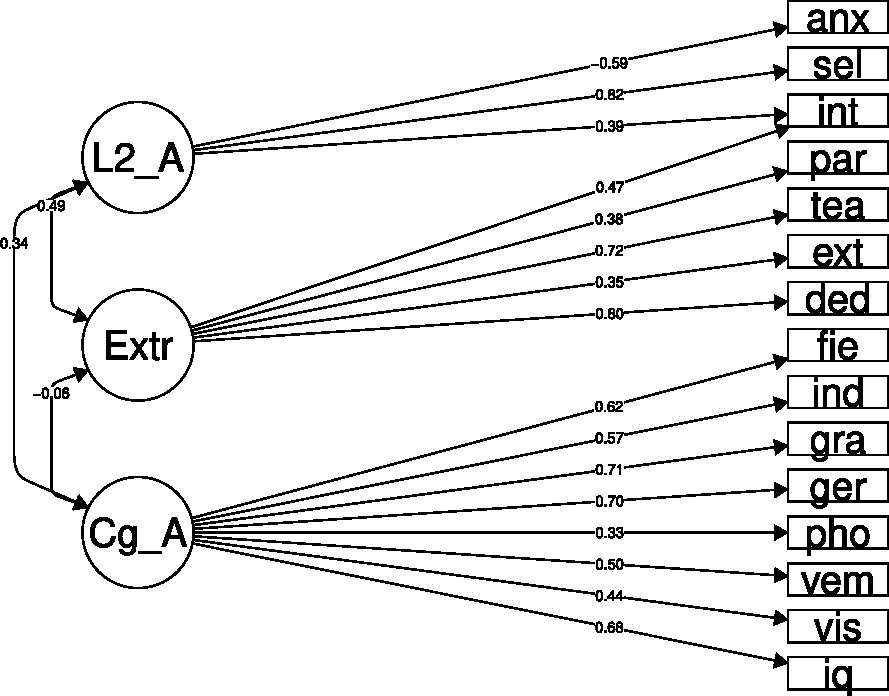
\includegraphics[width=\textwidth]{figures/Figure3.1.pdf}
\caption{\label{fig:03:1}Confirmatory factor analysis of the three-factor solution, variant 4; (L2\_A: L2 Academic Emotion; Extr: Extrinsic; Cg\_A: Cognition/Aptitude)}
\end{figure}

\subsection{Discussion of the Factor Analysis}

EFA was conducted with a sample of 174 L2 French learners (mean age 11.1). We then applied the structure to an independent sample of 615 L2 learners of English (mean age 10.5) by means of CFA to find out if the same structure could be uncovered in a different context and with a different target language. The EFA yielded three factors that were validated by the CFA: 1) Aptitude/Cognition, 2) Extrinsic Motivation, 3) L2 Academic Emotion. We will discuss these factors in turn.

The first factor (Aptitude/Cognition) regroups all cognitive and language-re\-lat\-ed ID variables. It explains most of the variance in the EFA model (16\%). The result suggests that for the young learners in this study, language-re\-lat\-ed and other cognitive variables are not clearly separable, but rather these abilities represent a common latent factor. Our data do not corroborate the presence of a language-specific dimension underlying these children’s instructed L2 learning. Rather, it provides evidence for a cognitive dimension involving language aptitude (phonetic coding, grammatical sensitivity, inductive ability), working memory (visual and verbal), intelligence, proficiency in language of instruction (in this case German), and field independence. This aligns with more recent conceptions of language learning ability that emphasize the complementarity of domain-specific and domain-general aspects (see e.g., \citealt{Skehan2019} for a discussion). Our data suggest that the language analysis component of aptitude and general cognitive ability are associated in young learners, a link that has so far been documented mainly for older learners (\citealt{Granena2012,Granena2012}; \citealt{Sasaki1996}). Moreover, language aptitude has been shown to be independent of, but overlapping with, intelligence in adults and adolescents (\citealt{WescheEtAl1982}; \citealt{Sasaki1996}; \citealt[827]{Li2016}). Our findings substantiate these claims for young learners. Having said that, both intelligence and language aptitude comprise several subcomponents and some authors argue that they are associated differently (\citealt{Granena2013}; \citealt{Li2016}). Since we did not assess all aspects of intelligence, we are unable to provide detailed information on the relationships between the various subcomponents.

Affective variables represent dimensions distinct from the cognitive and lan\-guage-re\-lat\-ed abilities. The two affective factors explain slightly less variance (12\% each). Factor 2 (labelled Extrinsic Motivation) is related to variables independent of the perceived qualities of the L2 as a school subject and includes extrinsic motivation, perceived teacher and parental encouragement, and dedication. Factor 3 (labelled L2 Academic Emotion) regroups emotions involved in L2 learning. These include enjoyment of L2 learning (intrinsic motivation), but also negative emotional states associated with it (anxiety), and children’s perception of themselves as L2 learners (self-concept). The interplay of these constructs is well documented in the literature (see Chapters 1 and 8). Learning processes in general are expected to trigger a range of emotions that mutually influence each other and ultimately impact on students’ academic achievement \citep{PekrunEtAl2002}. In terms of L2 learning, an unfavorable L2 self-concept may heighten anxiety experienced in the classroom, thus impacting negatively on a learner’s ability to enjoy L2 lessons and decrease intrinsic motivation. Several authors have described this connection: L2 anxiety has been found to correlate with learners’ motivational orientation in general \citep[189]{Heinzmann2013} and with intrinsic motivation in particular (\citealt{NoelsEtAl2000}; \citealt{Stoeckli2004}; \citealt{KormosCsizer2008}; \citealt{LiuHuang2011}). A reverse effect with poor language learning being the cause of anxiety has also been hypothesized \citep{SparksEtAl2011}. 

While the association between general cognitive abilities and aptitude variables emerged clearly from the data,there was some ambiguity associated with the affective variables \textit{locus of control} and i\textit{ntrinsic motivation} which loaded on both affective factors. The affective factors largely represent the distinction between intrinsic and extrinsic motivation from Self Determination Theory (SDT) by \citeauthor{DeciRyan1985} (\citeyear{DeciRyan1985, DeciRyan2002}; see Chapter 1 for a discussion). Intrinsic motivation is a central construct of SDT, subsuming self-determination, competence, and interpersonal relatedness as three basic psychological needs. Extrinsic motivation is present when an activity is engaged in to attain a separable outcome (\citealt[60]{DeciRyan2000}). The two types of motivation are closely linked, i.e. they are represented on a continuum, and extrinsic forms can gradually become intrinsic through the process of internalization (see e.g., \citealt{DeciRyan1985}). For instance, an external influence, such as expected career opportunities resulting from L2 learning, may be internalized, resulting in an intrinsic wish to study the language, provided that the individual feels in charge of the learning process (i.e. the need for self-determination is met). With regard to school learning,  \citet[64]{DeciRyan2000} emphasize that enjoyment of and willingness to engage with contents (intrinsic motivation) is shaped by teacher and peer interaction (external influence). The connection between the intrinsic and extrinsic dimension can be seen in our data from the double affiliation of intrinsic motivation with both affective factors. Indeed, when intrinsic motivation is allowed to load on two factors, the model fit becomes slightly better.

\section{Regression analysis}

We conducted a regression analysis with LAPS I and LAPS II. Due to the similarities of the findings, only LAPS II will be reported here.\footnote{The entire analysis is available at \url{https://osf.io/tpshc/}.} The aim of the regression analysis was to estimate the correlation between the three factors identified in the factor analysis and participants’ L2 English achievement. The dependent variable was the total score from the English test for listening and reading comprehension (OYLPT) taken at T1. \figref{fig:03:2} shows the bivariate associations of the scores in the data to which the statistical model was fitted.

  
\begin{figure}
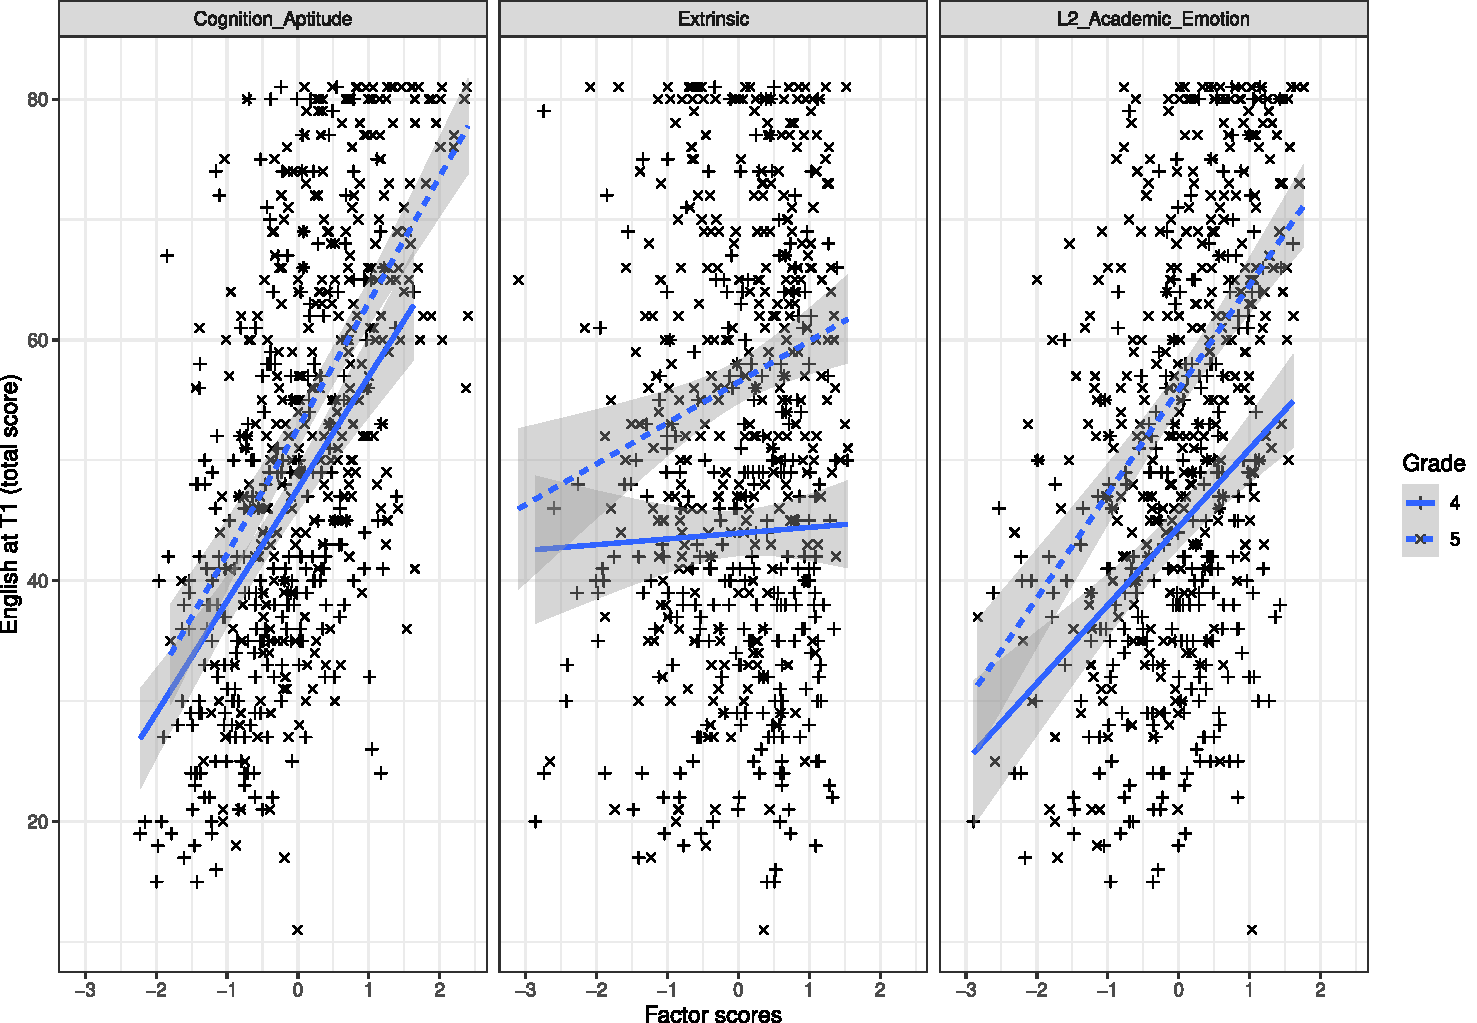
\includegraphics[width=\textwidth]{figures/Figure3.2.pdf}
\caption{\label{fig:03:2}Bivariate associations of the factor scores and English skills at T1 for grades 4 and 5 (LAPS II data). They indicate direction and strength of the relationship between each factor and L2 proficiency.}
\end{figure}

We fitted a linear mixed model with the lmer() function of the lme4 package \citep{BatesEtAl2015}. The factor scores from the CFA were introduced as independent variables (fixed effects). We included random intercepts by teacher to account for the clustered nature of the sample (random effects). 

As shown in \tabref{tab:03:3} and Figures~\ref{fig:03:2} and~\ref{fig:03:3}, Factor 1 (cognition/aptitude) and Factor 3 (L2 academic emotion) are positively correlated with L2 proficiency. The extrinsic Factor 2 is negatively correlated with L2 proficiency. These findings will be discussed in the next section. 


\begin{table}
\sisetup{table-space-text-post = {***}}
\caption{\label{tab:03:3}Summary of the regression model of the factor scores on English proficiency at T1}
\fittable{\begin{tabular}{l S[table-format=2.1]S[table-format=1.2]S[table-format=3.2]S[table-format=2.2]S[table-format=<1.3,table-align-text-post=false]} 
\lsptoprule
                    & {Estimate} & {SE} & {df} & {$t$} & {$\text{Pr}(>|t|)$}\\\midrule
(Intercept)         & 50.4 & 0.88 & 28.96 & 57.33 & < 0.001***\\
Cognition/aptitude  & 6.6 & 0.69 & 564.29 & 9.57 & < 0.001***\\
Extrinsic           & -6.9 & 1.06 & 582.92 & -6.51 & <0.001***\\
L2 academic emotion & 11.8 & 1.11 & 577.40 & 10.71 & < 0.001***\\
\lspbottomrule
\end{tabular}}
\end{table}
  
\begin{figure}
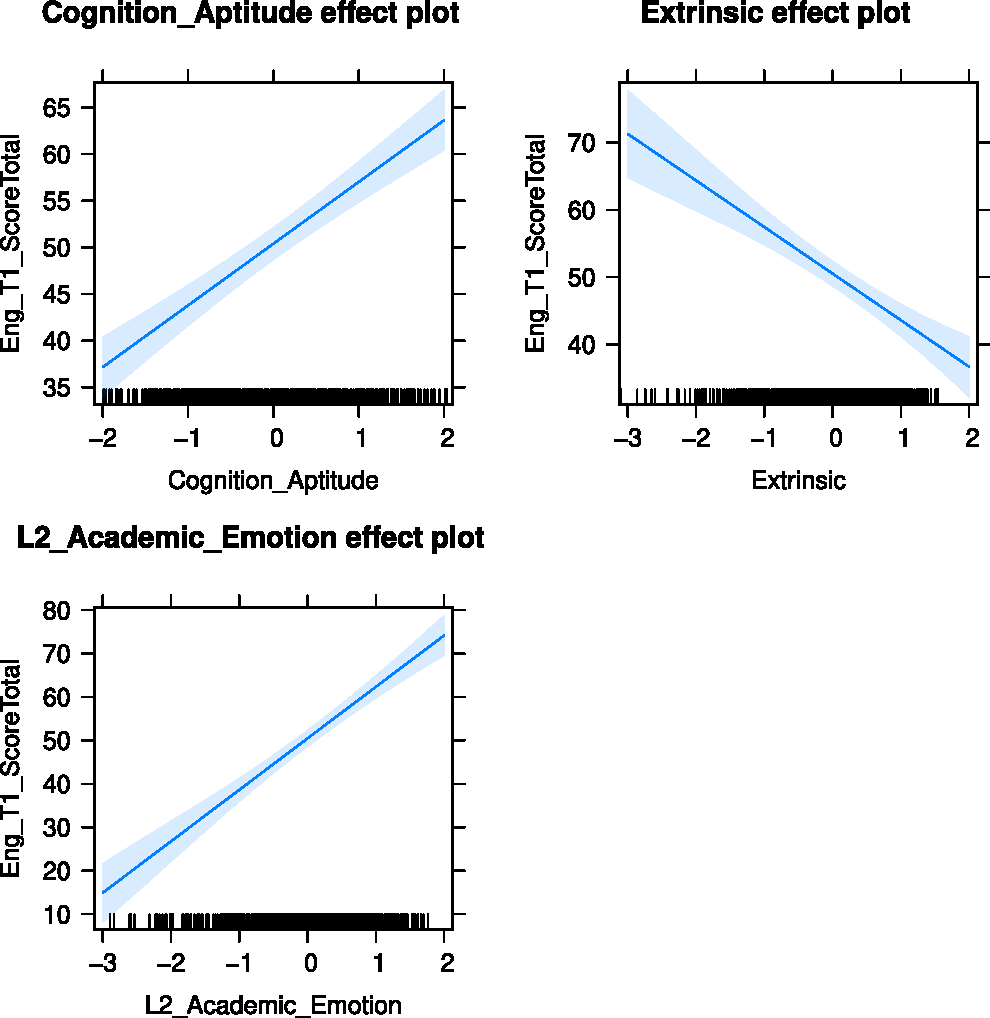
\includegraphics[width=.75\textwidth]{figures/Figure3.3.pdf}
\caption{\label{fig:03:3}Partial effects of the three factor scores and English skills at T1 (LAPS II data, both grades 4 and 5)}
\end{figure}

\subsection{Discussion of the regression analysis}

EFA and CFA yielded a robust factor structure with three factors: 1. cognition/aptitude, 2. extrinsic motivation, 3. L2 academic emotion. In the final step of the analysis, we were interested in the associations of these factors with L2 proficiency. To this aim, we considered:

\begin{enumerate}
\item the association between each individual factor and L2 proficiency illustrated in the bivariate correlation plots (\figref{fig:03:2})
\item and the mutual relationship between the three factors and L2 proficiency in a linear mixed model (\figref{fig:03:3}).
\end{enumerate}

\figref{fig:03:2} shows that the bivariate correlations between each factor and L2 proficiency are positive. When considered together in a mixed model (\figref{fig:03:3}), Factor 1 (Cognition/Aptitude) and Factor 3 (L2 Academic Emotion) are positively associated with L2 outcomes while Factor 2 (Extrinsic Motivation) is related negatively to L2 proficiency. This means that what remains of a statistical effect of Factor 2 on the outcome variable after controlling for the two other, more strongly associated constructs, is a negative effect. As some reviewers pointed out, the bivariate correlations and results from the regression analysis seem to contradict each other. It is worth noting that the two stand for different things: Bivariate associations show the correlation between two variables and indicate the direction and strength of the relationship between these two variables (e.g. between Factor 2 and L2 proficiency). Regression analysis, on the other hand, implies that an outcome depends on several variables that influence each other mutually. Regression aims to predict the outcome by considering these mutual influences. It is therefore possible for bivariate associations and the regression model to yield different tendencies.

Similar to our findings, other studies have documented weak or non-significant correlations between extrinsic motivation and L2 outcomes (\citealt[18]{HusfeldtLehmann2009}; \citealt[31]{KreisEtAl2014}). Also, negative effects for extrinsic motivation on L1 literacy have been reported, e.g., by \citet{WangGuthrie2004} for reading comprehension, \citet{BeckerEtAl2010} for reading, or by \citet{PajaresEtAl2009} for writing. These results can be interpreted with reference to the SDT framework (\citealt{DeciRyan2002}) which describes self-determination as a major driving force for achievement (see also Chapter 1, \sectref{sec:03:4.1}). Since extrinsic motivation is not usually related to self-determination, but rather stems from some external source, it is plausible that it impacts less on learning outcomes.

Several tentative conclusions can be drawn from our findings. A common factor for language aptitude and general learning abilities that is positively associated with L2 achievement implies that children with good results in cognitive tests are also good foreign language learners. This points to a kind of “allrounder” profile at primary school, and children who do well in foreign language classes are likely to be successful students in general. \citet{Pimsleur1966} may already have implied this as the PLAB included grades from subjects other than languages as an assessment criterion. Similarly, the data suggest that learners are unlikely to display difficulties related specifically and exclusively to foreign language instruction.

The effect of L2 Academic Emotion (anxiety, self-concepts and intrinsic motivation) on L2 outcomes is worth noting in relation to classroom practice. It highlights the importance of creating positive encounters with the target language that foster students’ enjoyment of L2 learning. This suggestion implies that ID variables that affect L2 achievement are dynamic and can be influenced by (adequate) learning conditions. While L2 motivation has been described as quite receptive to change (see also Chapter 8), the malleability of language aptitude, for instance, remains contested. Since components of language aptitude have emerged as vital players in children’s developing L2 competence in this chapter, as well as the predictive models (Chapter 4) and the variables underlying L1 German and L2 English development (Chapter 9), it would be worth knowing if they can be fostered to enhance foreign language learning. The stability of grammatical sensitivity and inductive ability has been investigated in the LAPS project and results are presented in Chapter 10.

\section{Conclusions}

We investigated the underlying structure of a broad set of ID variables involved in early instructed L2 learning. To this aim, a test battery of general learning abilities, language aptitude, and affective variables was administered to two different samples of primary school children aged 10--12 years. The research questions can be answered as follows:

\begin{description}
\item[Question 1:] What is the underlying structure of the ID variables, particularly in relation to language aptitude and general cognitive abilities? EFA yielded a 3 factor structure: Factor 1 subsumes general learning abilities and language aptitude and is named Cognition/Aptitude Factor. Factor 2 comprises extrinsic motivation, encouragement from adults and dedication. It is referred to as Extrinsic Motivation. Factor 3 involves emotions linked to L2 learning (intrinsic motivation, anxiety, and L2 self-concepts) and is therefore labelled L2 Academic Emotion. The model explains 40\% of the variance, with Factor 1 explaining 16\%, and Factors 2 and 3 contributing 12\% each.

\item[Question 2:] Is the structure replicable in an independent sample? The factor solution from the EFA was validated by means of CFA in an independent sample. This points to a robust factor structure, regardless of the population and target language. A distinction between language aptitude and general learning abilities was not supported by our data. Therefore, our results do not warrant for a special “language talent” that is independent of general cognitive abilities, nor do they indicate that some young learners are likely to struggle exclusively with foreign language instruction.

\item[Question 3:] What are the effects of the ID variables on L2 proficiency? A regression analysis with the 3 factors as predictors and L2 proficiency as the dependent variable shows that L2 achievement is positively associated with cognition/aptitude and L2 academic emotion. When these two factors are controlled for, the extrinsic factor has a negative effect on L2 achievement. 
\end{description}

Since findings from factor analysis cannot readily be generalized, we took care to provide conditions that maximize the informative value of our findings. Thus, we adopted a data-driven approach that included an exploratory and confirmatory analysis. Also, we selected two independent samples with – compared to other studies in the field of SLA – relatively large cohorts to optimize the validity of the factor structure. While the constructs assessed in the test battery remained unchanged, two tests pertaining to intelligence and phonetic coding ability were modified in accordance with advice from an expert panel. Also, L2 proficiency was operationalized differently in the two samples: as general language proficiency measured by C-Tests in LAPS I and as reading and listening comprehension in LAPS II. Results from the regression analysis were similar in both samples, suggesting a similar pattern of relationships between the three factors and different aspects of language proficiency. In the future, it would be interesting to extend to other areas, such as oral or written production. 

Understanding L2 learning for the age group investigated here seems a viable endeavor given the importance attached to early foreign language instruction in recent years. Therefore, we would encourage replications of the analyses presented in this chapter with samples from different populations learning different foreign languages. 

{\sloppy\printbibliography[heading=subbibliography,notkeyword=this]}
\end{document}
